\documentclass[conference]{IEEEtran}
\IEEEoverridecommandlockouts
% The preceding line is only needed to identify funding in the first footnote. If that is unneeded, please comment it out.
\usepackage{cite}
\usepackage{amsmath,amssymb,amsfonts}
\usepackage{algorithmic}
\usepackage{graphicx}
\usepackage{textcomp}
\usepackage{float} % for H placement option
\usepackage{listings}
\usepackage{xcolor}
\def\BibTeX{{\rm B\kern-.05em{\sc i\kern-.025em b}\kern-.08em
    T\kern-.1667em\lower.7ex\hbox{E}\kern-.125emX}}
\begin{document}

\title{Hard disk failure data analysis\\}

\author{\IEEEauthorblockN{Luca Falasca}
\IEEEauthorblockA{\textit{0334722} \\
luca.falasca@students.uniroma2.eu
}
\and
\IEEEauthorblockN{Matteo Conti}
\IEEEauthorblockA{\textit{0323728} \\
matteo.conti97@students.uniroma2.eu
}\\
}


\maketitle

\begin{abstract}
\end{abstract}

\section{Introduzione}
\subsection{Descrizione del problema}
Il problema da affrontare consiste nell'eseguire il batch processing di dati di grandi dimensioni mediante l'uso di una pipeline basata su framework Big Data. Nello specifico, l'obiettivo è analizzare un dataset contenente informazioni relative ai fallimenti dei dischi rigidi per l'esecuzione di 3 query di analisi dei dati e delle prestazioni di esse.

Il dataset fornito è una versione ridotta di quello presentato nel Grand Challenge della conferenza ACM DEBS 2024. Delle numerose colonne presenti nel dataset, ne sono state selezionate cinque per l'esecuzione delle query, in particolare:
\begin{itemize}
    \item \textbf{date}: data della misurazione
    \item \textbf{serial\_number}: identificativo del disco rigido
    \item \textbf{failure}: indica se il disco rigido ha avuto una failure o meno
    \item \textbf{model}: modello del disco rigido
    \item \textbf{vault\_id}: identificativo del gruppo di storage server
    \item \textbf{power\_on\_hours}: ore di accensione del disco rigido
\end{itemize}
\subsection{Obiettivi}
\section{Pipeline}
Per la gestione dei dati relativi ai guasti dei dischi rigidi, è stata implementata una pipeline ETL deployata in dei container docker. La pipeline è composta da diverse componenti, ognuna delle quali svolge un compito specifico, di seguito verranno analizzate le varie componenti della stessa.
\subsection{Data Ingestion}
Per la data ingestion è stato utilizzato il framework Apache NiFi, il quale permette di creare dei flussi di dati a partire da diversi tipi di sorgente, definire delle operazioni di trasformazione sui flussi di dati e andare a memorizzare il risultato delle trasformazioni su datastore di diverso tipo. Nel nostro caso NiFi svolge le seguenti operazioni:
\begin{enumerate}
    \item Riceve tramite HTTP il file CSV contenente i dati relativi ai guasti dei dischi rigidi
    \item Effettua una query SQL (Figura \ref{fig:nifi_query}) per selezionare solamente le cinque colonne di interesse del CSV ed effettuare pulizia dei dati rimuovendo righe contenenti valori nulli o invalidi
    \item Effettua l'assegnazione esplicita dello schema ai dati
    \item Scrive i dati su HDFS in formato Parquet e CSV
\end{enumerate}
\begin{figure}[H]
    \centering
    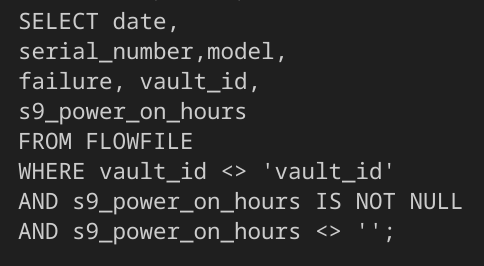
\includegraphics[width=0.4\textwidth]{./res/query_nifi.png}
    \caption{Query SQL filtraggio dati NiFi}
    \label{fig:nifi_query}
\end{figure} 
\subsection{Data Storage}
Come data lake in cui memorizzare i dati a a seguito del preprocessamento effettuato da parte di NiFi è stato utilizzato HDFS, il quale permette di memorizzare grandi quantità di dati su un cluster di nodi. Nel nostro caso il cluster è composto da:
\begin{itemize}
    \item 1 NameNode
    \item 2 DataNode
\end{itemize}
Non è stata utilizzata una struttura particolare per l'organizzazione dei file all'interno di HDFS, i file sono stati memorizzati tutti nella root directory. 
\subsection{Data Processing}
Per il processamento dei dati e quindi l'esecuzione delle query è stato utilizzato il framework Spark, in particolare utilizzando la versione per python PySpark.Per queste query è stato utilizzato un cluster composto da uno spark master e quattro spark worker. Per farlo abbiamo utilizzato l'immagine bitami/spark nella versione 3.5.1. Per l'orchestrazione del cluster abbiamo utilizzato docker compose.
Il dataset parzialemente filtrato è stato caricato dall'hdfs e i risultati delle query sono stati salvati in mongodb utilizzando il connettore spark-mongodb.
Le query sono state eseguite sia a partire da file in formato CSV che in formato Parquet per valutare le differenze di prestazioni tra un formato basato su colonne e uno basato su righe.
\subsubsection{Query 1}
\subsubsection{Query 2}
\subsubsection{Query 3}
\subsection{Analytical Data Storage}
I risultati delle query sono stati memorizzati in un database MongoDB (Fig. \ref{fig:mongo}).
Per organizzare i dati, abbiamo creato una collezione per ciascuna query, dove ogni documento rappresenta una riga dei risultati ottenuti dalla query stessa. Inoltre, abbiamo un'altra collezione che contiene i risultati, includendo il timestamp dell'esperimento, la query specifica e il formato con cui è stata eseguita, oltre al tempo impiegato per l'esecuzione.

\begin{figure}[htbp]
    \centerline{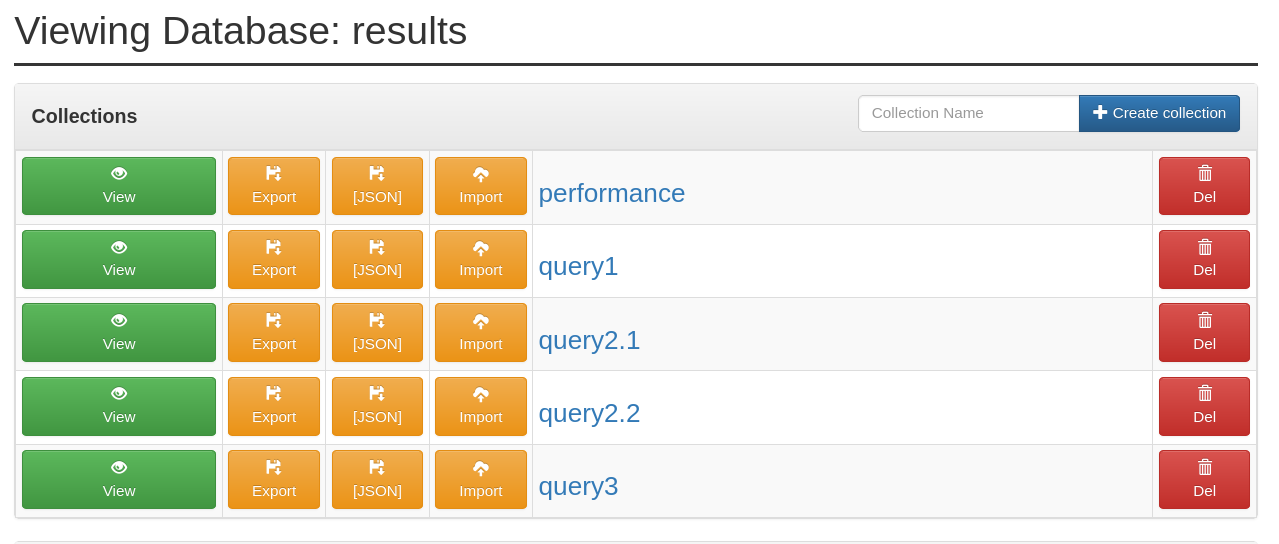
\includegraphics[width=0.5\textwidth]{res/mongo.png}}
    \caption{Schema del database MongoDB.}
    \label{fig:mongo}
\end{figure}
\subsection{Visualization}
\subsection{Analisi delle prestazioni}
\vspace{12pt}


\end{document}

    